\documentclass[aspectratio=169,10pt]{beamer}
% Compile with pdfLaTeX. Keep the supplied images folder beside this file.
\usepackage{tikz}
\usepackage[T1]{fontenc}
\usepackage[utf8]{inputenc}
\usepackage{lmodern}
\usepackage{amsmath,amssymb,booktabs,graphicx,array,tabularx}
\usetheme{Madrid}
\definecolor{ProjectBlue}{RGB}{51,51,179}
\setbeamercolor{structure}{fg=ProjectBlue}
\setbeamercolor{normal text}{fg=black,bg=white}
\setbeamercolor{frametitle}{fg=white,bg=ProjectBlue}
\setbeamercolor{framesubtitle}{fg=white}
\setbeamercolor{author in head/foot}{fg=white,bg=ProjectBlue}
\setbeamercolor{title in head/foot}{fg=white,bg=ProjectBlue}
\setbeamercolor{date in head/foot}{fg=white,bg=ProjectBlue}
\setbeamerfont{frametitle}{size*= {17}{20}}
\setbeamerfont{framesubtitle}{size*= {9.5}{11}}
\setbeamertemplate{itemize item}[ball]
\setbeamertemplate{itemize subitem}[circle]
\setbeamertemplate{navigation symbols}{}
\setbeamersize{text margin left=0.45cm,text margin right=0.45cm}
\setbeamertemplate{footline}{%
  \leavevmode\hbox{%
  \begin{beamercolorbox}[wd=.20\paperwidth,ht=2.5ex,dp=1ex,center]{author in head/foot}
    \fontsize{6.2}{7}\selectfont NU Mathematics
  \end{beamercolorbox}%
  \begin{beamercolorbox}[wd=.52\paperwidth,ht=2.5ex,dp=1ex,center]{title in head/foot}
    \fontsize{6.2}{7}\selectfont Kazakhstan electricity forecasting
  \end{beamercolorbox}%
  \begin{beamercolorbox}[wd=.28\paperwidth,ht=2.5ex,dp=1ex,center]{date in head/foot}
    \fontsize{6.2}{7}\selectfont 24 November 2026\hspace{1em}\insertframenumber/\inserttotalframenumber
  \end{beamercolorbox}}}
\graphicspath{{images/}}
\setbeameroption{hide notes}
% Replace the preceding line with the next line to print the speaking scripts:
% \setbeameroption{show only notes}
\newcommand{\Source}[1]{\par\vfill{\fontsize{6.5}{7.5}\selectfont\color{black!65}#1\par}}
\newcommand{\SmallTable}{\fontsize{9}{10.5}\selectfont}
\title{Forecasting Kazakhstan's Total Monthly Electricity Generation Using SARIMA}
\author{Narlen Ualikan, Dariya Kuantay, Aibek Tumenbayev, Azhar Sarbassova}
\institute{Nazarbayev University}
\date{24 November 2026}


\begin{document}
% Four speakers: slides 1--3, 4--6, 7--9, 10--12; backups follow.
\begin{frame}[t]{Forecasting electricity generation}
\framesubtitle{Kazakhstan's national monthly total}
\par\medskip
{\Large\bfseries Seasonal forecasts with and without a growth adjustment\par}
\par\medskip
Narlen Ualikan, Dariya Kuantay,\\Aibek Tumenbayev, Azhar Sarbassova\par
Nazarbayev University
\par\bigskip
\textbf{Question:} Does the selected SARIMA improve three-month forecasts over simple seasonal benchmarks?
\par\medskip\par
\textbf{Target:} national monthly generation in terawatt-hours (TWh).
\Source{Historical test on a frozen Ember snapshot. Original comparison retained; growth-adjusted benchmark added as a follow-up.}
\note{Person 1, slide 1. We forecast Kazakhstan's total monthly electricity generation in terawatt-hours. We compare SARIMA with two simple seasonal rules. Our original project compared SARIMA with repeating last year's corresponding month. The original results showed underprediction during a year of growth, so we added a fixed adjustment for recent annual change. We present this addition transparently as a follow-up comparison. It uses no observations after each forecast cutoff, but it is not a new independent test because we had already seen the original test results.}
\end{frame}

\begin{frame}[t]{Dataset and seasonal pattern}
\framesubtitle{Ember monthly electricity data}
\textbf{Full snapshot:} 102 months, January 2018--June 2026.\par
\textbf{Main study:} 84 months, January 2019--December 2025.
\begin{center}
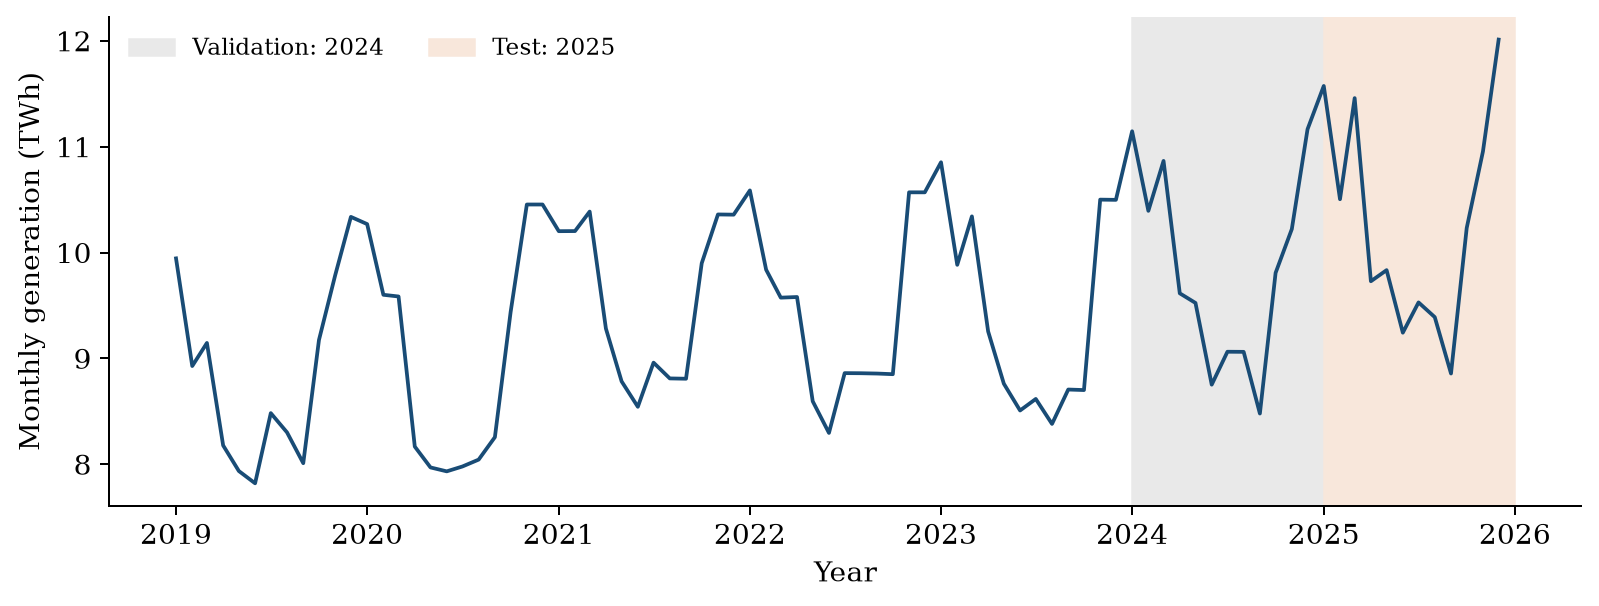
\includegraphics[width=.96\linewidth,height=4.65cm,keepaspectratio]{01_history.png}
\end{center}
\textbf{Pattern:} recurring annual variation; national generation is distinct from demand.
\Source{Ember, snapshot downloaded 18 November 2026. The display includes all study years; exploration uses 2019--2023 only.}
\note{Person 1, slide 2. Ember is the public source. We select Kazakhstan and total generation rather than an individual company's plants. The complete snapshot contains 102 monthly observations, with no missing months or duplicate dates. Our experiment uses complete years from 2019 through 2025, leaving the partial 2026 year outside the main evaluation. The historical pattern supports a seasonal forecast comparison. A full-series plot describes the data; only the initial training years informed exploration and stationarity checks. These are revised snapshot values, not the data vintages available at the historical dates.}
\end{frame}

\begin{frame}[t]{2018 source audit}
\framesubtitle{Repeated values suggest averaging, but do not prove it}
Ember reports \textbf{9.780 TWh in each of January, February and March 2018}.
\begin{center}
\begin{tabular}{lrr}\toprule
2018 period & Ember (TWh) & Samruk (TWh)\\\midrule
January & 9.7800 & 10.3573\\
January--March total & 29.3400 & 29.3392\\\bottomrule
\end{tabular}
\end{center}
\begin{itemize}
\item January differs from the original national source table.
\item The quarterly totals nearly match: quarterly averaging is plausible.
\item This check does not establish the construction of every monthly value.
\end{itemize}
\textbf{Decision:} exclude 2018 in the main experiment; add it back without retuning.
\Source{Frozen Ember CSV and original Samruk January / Q1 2018 DOCX tables. Other repeated values remain; no manual corrections.}
\note{Person 1, slide 3. Complete data can still have measurement issues. Ember repeats exactly 9.780 for each of the first three months of 2018. Samruk's original national table gives 10.3573 for January, so the January values disagree. The first-quarter totals, however, almost match. That pattern is consistent with averaging a quarterly total into equal monthly observations, but our check cannot prove the rule for every month. We preserve the data, exclude 2018 in the main analysis and add it back in a sensitivity check. Person 2 will explain the evaluation design.}
\end{frame}

\begin{frame}[t]{Chronological evaluation}
\framesubtitle{Model choice precedes the 2025 test}
\begin{center}
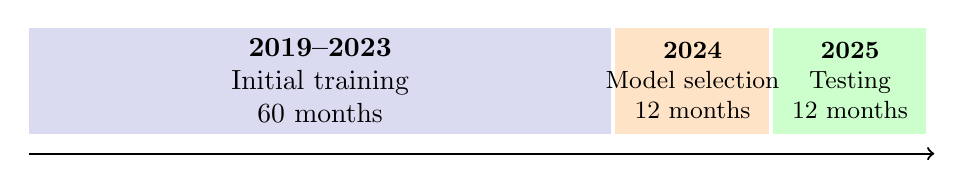
\begin{tikzpicture}[x=1cm,y=1cm]
\fill[ProjectBlue!18] (0,0) rectangle (7.4,1.35);
\fill[orange!22] (7.45,0) rectangle (9.4,1.35);
\fill[green!20] (9.45,0) rectangle (11.4,1.35);
\node[align=center] at (3.7,.68) {\textbf{2019--2023}\\Initial training\\60 months};
\node[align=center,font=\small] at (8.43,.68) {\textbf{2024}\\Model selection\\12 months};
\node[align=center,font=\small] at (10.43,.68) {\textbf{2025}\\Testing\\12 months};
\draw[->,thick] (0,-.25)--(11.5,-.25);
\end{tikzpicture}
\end{center}
\begin{itemize}
\item Select SARIMA using four three-month blocks in 2024.
\item Freeze its order; refit parameters with expanding histories in 2025.
\item Test blocks: \textbf{Jan--Mar, Apr--Jun, Jul--Sep, Oct--Dec}.
\item All three models forecast the same targets and horizons 1, 2 and 3.
\end{itemize}
No actual value from inside a forecast block enters that block's forecasts.
\Source{The fixed growth rule is a follow-up, not selected on 2024 or tuned on 2025.}
\note{Person 2, slide 4. This timeline separates the three jobs. The first five years provide initial training. The following year selects the SARIMA specification using forecast errors. We then freeze the selected order for the 2025 test, but refit its parameters when another three months of observations become available. All models forecast exactly the same four blocks at the same horizons. At the start of a block, its next three actual values are unavailable. After a block ends, those observed values can enter the next fit. This prevents information from the future entering a block's forecasts.}
\end{frame}

\begin{frame}[t]{Three forecast methods}
\framesubtitle{A fixed additive growth rule makes the baseline more demanding}
\begin{enumerate}
\item \textbf{Seasonal naive:} repeat each matching month from last year.
\item \textbf{Growth-adjusted seasonal naive:} add the average year-on-year change over the latest 12 observed months. Use one adjustment for all three forecasts.
\item \textbf{SARIMA$(1,0,0)(0,1,1)_{12}$ with a constant:} retain the original 2024 selection and 2025 refitting procedure.
\end{enumerate}
\par\medskip
\textbf{Follow-up status:} the growth benchmark was prompted by the original results. Its additive form and 12-month window are fixed; no alternatives are tuned on the test.
\Source{Growth means an absolute TWh change, not a percentage. Equations and full candidate comparison are in backup slides.}
\note{Person 2, slide 5. The original seasonal naive rule simply repeats last year's matching months. The new rule also repeats those months but adds a recent average annual change measured in terawatt-hours. We calculate twelve year-on-year differences from observed data and average them. At a given cutoff that same adjustment is used for all three forecast months. This is an additive adjustment, not a percentage growth rate. The SARIMA specification and refitting procedure remain unchanged. We did not search different windows or growth definitions to improve the test score.}
\end{frame}

\begin{frame}[t]{April 2025 forecast block}
\framesubtitle{Fit through March; issue April--June forecasts together}
\textbf{Cutoff: March 2025.} No April--June actual values enter these forecasts.
\begin{center}
\SmallTable
\begin{tabularx}{\linewidth}{@{}Xrrrr@{}}\toprule
Month & Actual & Naive & Growth-adjusted & SARIMA\\
\midrule
April & 9.729 & 9.615 & 10.023 & 9.978\\
May & 9.834 & 9.524 & 9.932 & 9.455\\
June & 9.243 & 8.752 & 9.160 & 8.981\\
\bottomrule\end{tabularx}

\end{center}
\textbf{Growth adjustment:} 0.407833 TWh for \emph{all three} months.\par
April: 9.615 + 0.407833 $\approx$ 10.023 TWh.
\par\medskip\par
After scoring the block, April--June observations may enter the July fit.
\Source{All table values are TWh. The adjustment averages April 2024--March 2025 changes against April 2023--March 2024.}
\note{Person 2, slide 6. Here is one complete block. We fit through March 2025 and forecast April, May and June together. The table compares the actual totals, revealed later, with each model's forecasts. The growth adjustment is about 0.408 terawatt-hours. It is computed from the latest twelve observed annual changes, so we add the same amount to the three corresponding 2024 values. For example, April's 9.615 becomes approximately 10.023. We do not use April's actual generation to revise May or June. Person 3 will now present the full test comparison.}
\end{frame}

\begin{frame}[t]{2025 forecasts and model comparison}
\framesubtitle{Growth-adjusted naive has the lowest pooled errors in this test}
\vspace{-.15cm}
\begin{center}
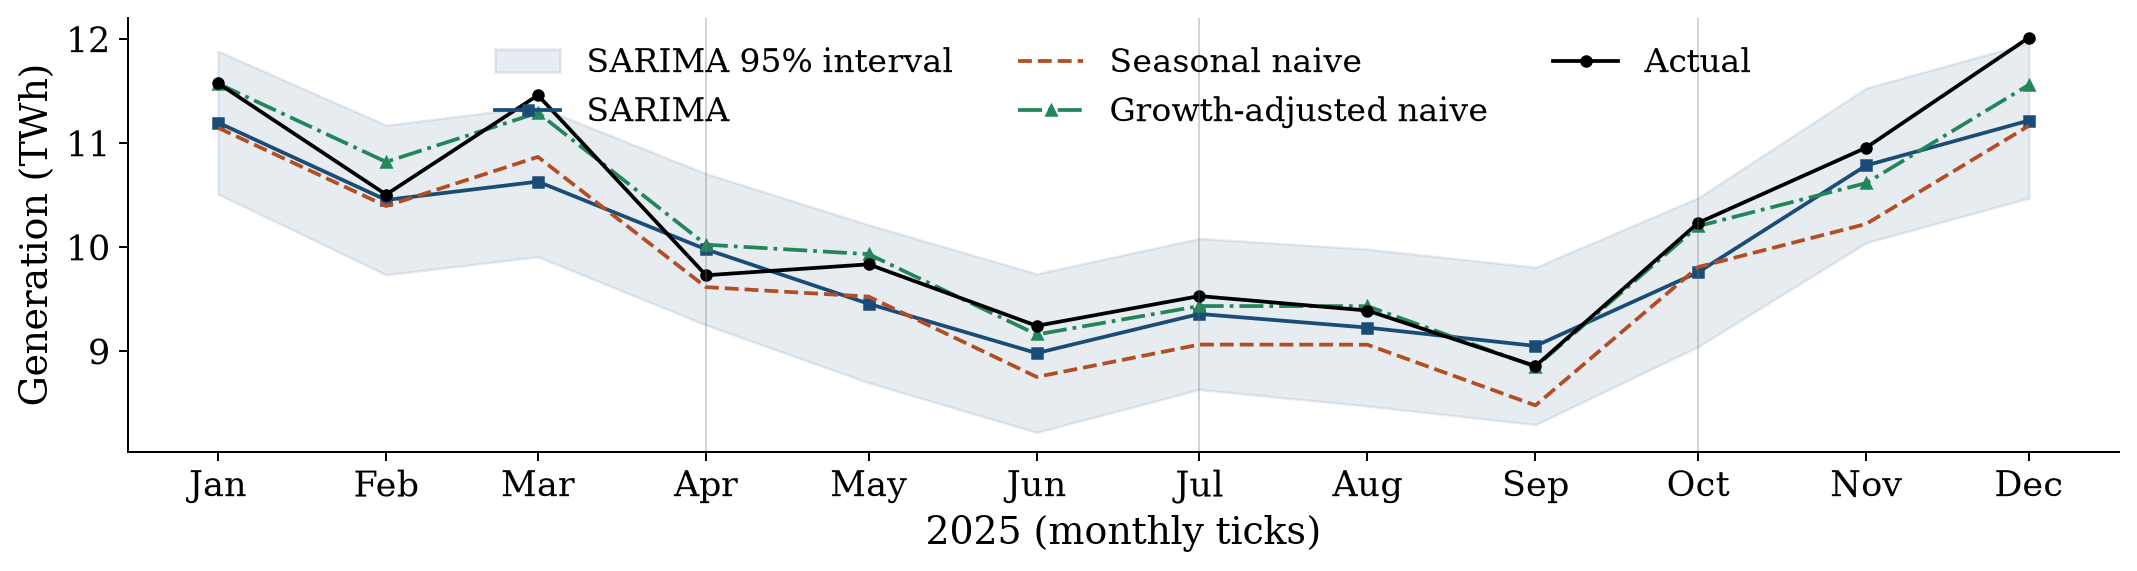
\includegraphics[width=.97\linewidth,height=3.8cm,keepaspectratio]{06_test_slide.png}
\vspace{-.15cm}\par
\SmallTable
\begin{tabularx}{\linewidth}{@{}Xrrr@{}}\toprule
Model & MAE (TWh) & RMSE (TWh) & Mean error (TWh)\\
\midrule
Seasonal naive & 0.435 & 0.483 & 0.435\\
Growth-adjusted naive & 0.161 & 0.217 & 0.036\\
SARIMA & 0.343 & 0.418 & 0.270\\
\bottomrule\end{tabularx}

\end{center}
\textbf{SARIMA beats the original baseline, but not the growth-adjusted benchmark.}
\Source{All errors are TWh; mean error = actual minus forecast. Twelve test values; four origins. Shading: SARIMA 95\% interval. Growth comparison is a follow-up.}
\note{Person 3, slide 7. This is our main result. The graph displays all three forecast paths against actual generation. Monthly ticks are separate from the quarterly refitting boundaries. The table pools the twelve errors, including four forecasts at each horizon. The original scores reproduce exactly: seasonal naive has MAE 0.435 and SARIMA has 0.343. The growth-adjusted rule has MAE 0.161 and RMSE 0.217, both lower than SARIMA. Its mean error is also closer to zero. Therefore our revised conclusion is that SARIMA beats the original baseline but does not beat this more demanding benchmark on 2025.}
\end{frame}

\begin{frame}[t]{Errors by forecast horizon}
\framesubtitle{Only four forecasts contribute to each horizon}
\begin{center}
\SmallTable
\begin{tabularx}{\linewidth}{@{}Xrrrr@{}}\toprule
Horizon & Count & Naive MAE & Growth-adjusted MAE & SARIMA MAE\\
\midrule
1 & 4 & 0.358 & 0.106 & 0.318\\
2 & 4 & 0.370 & 0.199 & 0.191\\
3 & 4 & 0.577 & 0.179 & 0.520\\
\bottomrule\end{tabularx}

\end{center}
\begin{itemize}
\item Growth-adjusted naive has lower MAE at horizons 1 and 3.
\item SARIMA is slightly better at horizon 2: 0.191 versus 0.199 TWh.
\item The pooled ranking does not imply a win at every horizon or origin.
\end{itemize}
\Source{MAE in TWh. Each row has four observations; individual months can strongly affect the ranking.}
\note{Person 3, slide 8. These are the errors separated by forecast horizon. Each row contains only four observations, one from each origin. The growth-adjusted rule performs best at horizons one and three. SARIMA has slightly lower error at the second month, about 0.191 compared with 0.199 for the growth benchmark. This distinction matters: a better pooled score does not mean a model is better everywhere. Four observations per row are also too few for a strong general conclusion. We report the observed differences rather than claiming statistical significance.}
\end{frame}

\begin{frame}[t]{Sensitivity to including 2018}
\framesubtitle{Same selected SARIMA specification; no retuning}
\begin{center}
\begin{tabular}{lrr}\toprule
2025 comparison & MAE (TWh) & RMSE (TWh)\\\midrule
Original seasonal naive & 0.435 & 0.483\\
Growth-adjusted naive & 0.161 & 0.217\\
SARIMA, main sample & 0.343 & 0.418\\
SARIMA, including 2018 & 0.360 & 0.441\\\bottomrule
\end{tabular}
\end{center}
\begin{itemize}
\item Both naive rules are unchanged: their required recent data exclude 2018.
\item SARIMA still beats the original baseline, but not the growth-adjusted rule.
\item This sensitivity does not resolve the construction of repeated monthly values.
\end{itemize}
\Source{Same targets, cutoffs and horizons. Adding 2018 changes SARIMA's history, not its specification.}
\note{Person 3, slide 9. We also add 2018 back to the history without selecting the model again. SARIMA's test MAE becomes about 0.360, slightly worse than in the main experiment. The two naive forecasts are unchanged because their inputs involve only much more recent months. The growth-adjusted rule therefore still has the lowest pooled error. This sensitivity preserves the main ranking, but it does not fix the source issue or establish that all the monthly values are accurate. Person 4 will explain the uncertainty and the limits of the conclusion.}
\end{frame}

\begin{frame}[t]{Prediction uncertainty}
\framesubtitle{Better point forecasts do not establish calibrated intervals}
\begin{center}
\begin{tabular}{lrr}\toprule
SARIMA interval & Covered observations & Observed coverage\\\midrule
Nominal 80\% & 9 of 12 & 75.0\%\\
Nominal 95\% & 10 of 12 & 83.3\%\\\bottomrule
\end{tabular}
\end{center}
\begin{itemize}
\item Coverage is below nominal levels on this small test set.
\item Pre-test residual checks detect no autocorrelation at the tested lags.
\item Non-rejection does not prove correct specification or reliable intervals.
\end{itemize}
No prediction intervals are claimed for the added growth benchmark.
\Source{SARIMA intervals are conditional Gaussian intervals. Detailed residual plots, coefficients and tests are in backups.}
\note{Person 4, slide 10. We keep the original prediction interval results. The nominal eighty percent intervals cover nine of the twelve actual values. The nominal ninety-five percent intervals cover ten. Coverage is therefore below the nominal levels, although twelve observations cannot precisely estimate long-run coverage. Pre-test residual tests do not detect autocorrelation at the selected lags, but that does not prove the model or its uncertainty estimates are correct. We do not invent prediction intervals for the new benchmark, which is evaluated only for point forecasts.}
\end{frame}

\begin{frame}[t]{Limits of the comparison}
\framesubtitle{One test year, four origins and a follow-up benchmark}
\begin{itemize}
\item The growth adjustment addresses recent annual increases; it may fail if growth reverses.
\item The rule was added after seeing the original results: a new period is needed for an independent test.
\item A frozen revised snapshot differs from real-time historical data vintages.
\item Only part of the source chain was audited; repeated values remain.
\item Weather, outages, fuel supply and trade are outside the univariate models.
\end{itemize}
\par\medskip
\textbf{Next step:} freeze all three methods and assess more forecast origins.
\Source{The observed ranking is descriptive. It does not establish statistical significance, causation or permanent superiority.}
\note{Person 4, slide 11. The new rule is useful because it adjusts a simple seasonal forecast for recent annual increases. That mechanism may not work when growth slows or reverses. We also acknowledge that the benchmark was prompted by the original results, so its strong test score is a follow-up finding. A fresh period would be needed for a more independent assessment. The data are a frozen revised snapshot and the source audit covers only part of the series. External influences are not modeled. Our next step would be to freeze these methods and evaluate more origins.}
\end{frame}

\begin{frame}[t]{Conclusion}
\framesubtitle{Did SARIMA outperform the growth-adjusted benchmark?}
\par\bigskip
{\Large\bfseries No, on the 2025 test it did not.\par}
\par\bigskip
\textbf{Pooled MAE:} growth-adjusted naive \textbf{0.161 TWh};\\SARIMA \textbf{0.343 TWh}.
\par\medskip\par
Growth adjustment gives 53.1\% lower MAE than SARIMA.\par
SARIMA's 21.1\% improvement survives only against the original naive rule.
\par\bigskip
The stronger baseline changes the interpretation of the original finding.\par
The conclusion remains limited to this small historical follow-up comparison.
\Source{Same four forecast blocks; no change to SARIMA selection. Thank you.}
\note{Person 4, slide 12. Our direct answer is no. SARIMA does not outperform the growth-adjusted seasonal naive benchmark on the 2025 test. The growth rule has pooled MAE 0.161 terawatt-hours, compared with 0.343 for SARIMA. SARIMA still improves on the original seasonal naive baseline, so the original scores were reproducible. What changes is the interpretation: outperforming a baseline that ignores recent growth is not sufficient evidence of an advantage over a slightly stronger simple method. This is a limited historical follow-up, and a fresh evaluation would strengthen the evidence. Thank you.}
\end{frame}

\appendix
\begin{frame}[t]{Backup: Full 2024 candidate comparison}
\framesubtitle{Selection remains based on validation MAE}
\begin{center}
\SmallTable
\begin{tabularx}{\linewidth}{@{}Xrrr@{}}\toprule
Specification, period 12 & Constant & MAE (TWh) & Initial AICc\\
\midrule
(1,0,0)(0,1,1) & Yes & 0.354 & 50.70\\
(0,0,1)(0,1,1) & Yes & 0.358 & 53.74\\
(1,0,1)(0,1,1) & Yes & 0.378 & 50.08\\
(1,0,0)(1,1,0) & Yes & 0.400 & 52.78\\
(1,1,0)(0,1,1) & No & 0.411 & 53.42\\
(0,1,1)(0,1,1) & No & 0.429 & 48.13\\
(1,1,0)(1,1,0) & No & 0.456 & 56.82\\
(0,1,1)(1,1,0) & No & 0.465 & 50.61\\
\bottomrule\end{tabularx}

\end{center}
\small Minimum unrounded validation MAE. Exact ties use AICc only if all tied models share $(d,D)$; otherwise retain original candidate enumeration. \textbf{No tie occurred.}
\Source{AICc values across different differencing orders are descriptive only. Seasonal naive validation MAE: 0.508 TWh.}
\end{frame}

\begin{frame}[t]{Backup: Pre-test coefficient estimates}
\framesubtitle{Selected SARIMA fitted through December 2024}
\begin{center}
\SmallTable
\begin{tabularx}{\linewidth}{@{}Xrr@{}}\toprule
Parameter & Estimate & Std. error\\
\midrule
Constant $c$ & 0.1214 & 0.0313\\
AR $\phi$ & 0.3138 & 0.1409\\
Seasonal MA $\theta$ & -0.8640 & 0.3788\\
Innovation variance ($\mathrm{TWh}^2$) & 0.1162 & 0.0328\\
\bottomrule\end{tabularx}

\end{center}
\par\medskip
The constant is an intercept for year-on-year change, not its unconditional mean.\par
These are pre-test coefficients, not every quarterly refit's estimates.
\Source{Maximum likelihood; asymptotic standard errors. All fits converged.}
\end{frame}

\begin{frame}[t]{Backup: Forecast equations}
\framesubtitle{At cutoff $T$; horizons $h=1,2,3$}
\textbf{Seasonal naive:}\quad $\widehat y_{T+h\mid T}=y_{T+h-12}.$
\par\medskip\par
\textbf{Growth-adjusted naive:}
\[
g_T=\frac1{12}\sum_{j=0}^{11}(y_{T-j}-y_{T-j-12}),\qquad
\widehat y^{\mathrm{growth}}_{T+h\mid T}=y_{T+h-12}+g_T.
\]
\textbf{Selected SARIMA:}\quad $z_t=y_t-y_{t-12}$,
\[
z_t=c+\phi z_{t-1}+\varepsilon_t+\theta\varepsilon_{t-12}.
\]
\textbf{Scores:}\quad $e_i=y_i-\widehat y_i$,
\quad $\mathrm{MAE}=n^{-1}\sum_i|e_i|$,
\quad $\mathrm{RMSE}=\sqrt{n^{-1}\sum_i e_i^2}$.
\Source{Growth is an additive absolute TWh change. Use only observations through cutoff T; same adjustment at all three horizons.}
\end{frame}

\begin{frame}[t]{Backup: Residual diagnostics}
\framesubtitle{Pre-test fit only; omit the first 13 residuals}
\begin{center}
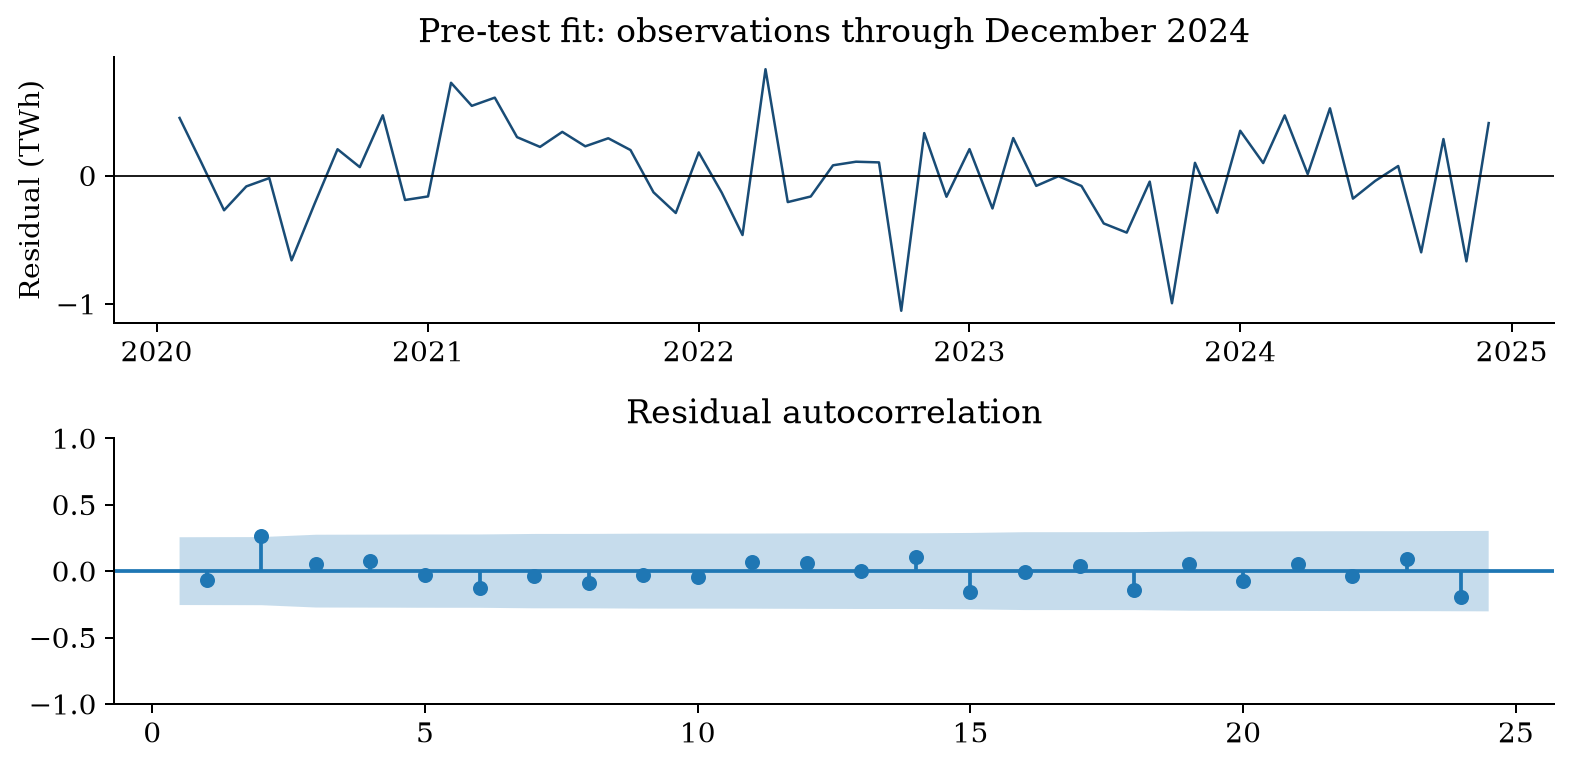
\includegraphics[width=.94\linewidth,height=4.6cm,keepaspectratio]{05_residuals.png}
\end{center}
\small Ljung--Box: lag 12 statistic 8.075, $p=0.621$; lag 24 statistic 18.888, $p=0.652$. Two AR/MA degrees of freedom removed; residual mean 0.016 TWh.
\Source{Non-rejection does not establish independence, normality, constant variance or correct specification.}
\end{frame}

\begin{frame}[t]{Backup: Stationarity and correlation}
\framesubtitle{Initial training sample, 2019--2023}
\begin{center}
\SmallTable
\begin{tabular}{lrrr}\toprule
Series & $n$ & ADF $p$ & KPSS $p$\\\midrule
Levels & 60 & 0.186 & $\geq0.100$\\
Seasonal difference & 48 & 0.0008 & 0.095\\
Seasonal and first difference & 47 & $<0.001$ & $\geq0.100$\\\bottomrule
\end{tabular}\par
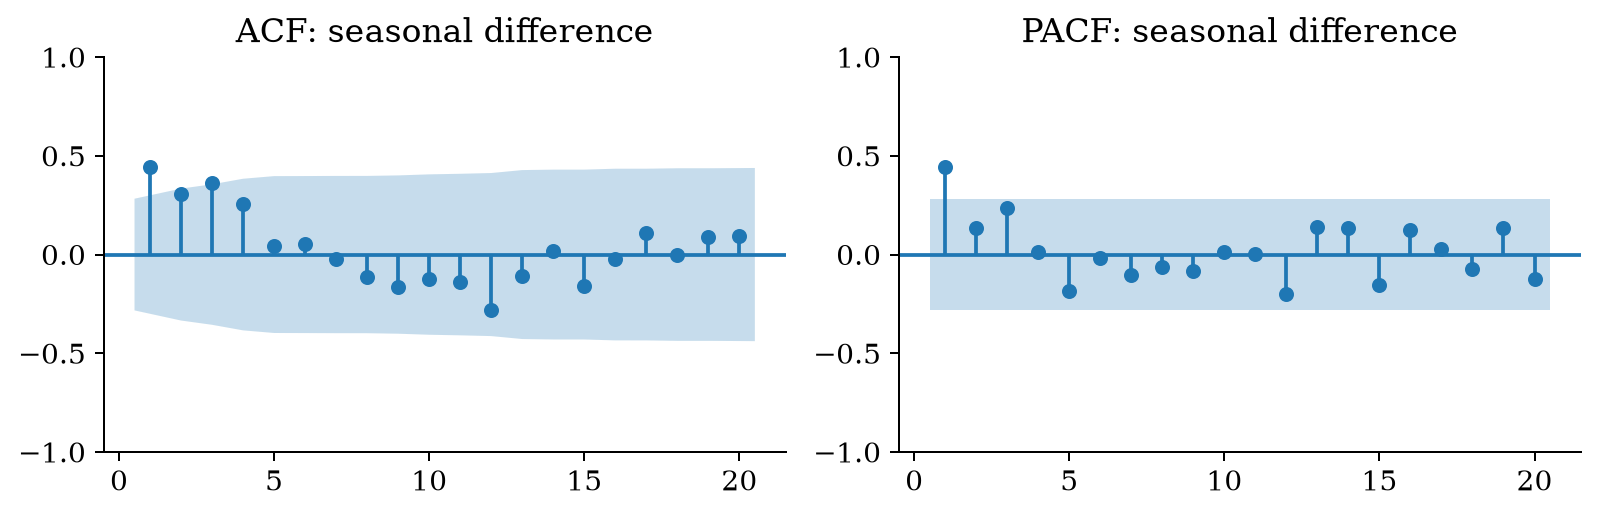
\includegraphics[width=.94\linewidth,height=3.4cm,keepaspectratio]{03_acf_pacf.png}
\end{center}
\Source{ADF: unit-root null, constant, AIC lags up to 8. KPSS: level-stationarity null, automatic bandwidth. Levels are inconclusive; table-limit p-values are bounds.}
\end{frame}

\begin{frame}[t]{Backup: Dated forecast illustration}
\framesubtitle{Selected SARIMA; information through December 2025}
\begin{center}
\begin{tabular}{lrrr}\toprule
Month & Forecast & 95\% lower & 95\% upper\\\midrule
January 2026 & 11.860 & 11.130 & 12.590\\
February 2026 & 10.812 & 10.052 & 11.572\\
March 2026 & 11.367 & 10.605 & 12.129\\\bottomrule
\end{tabular}
\end{center}
All values are TWh. These are dated historical forecasts, not live November 2026 forecasts, and do not enter selection or test scores.
\Source{No later 2026 observations enter this fit.}
\end{frame}

\begin{frame}[t]{Backup: Data and references}
\framesubtitle{Frozen inputs and reproducible methods}
\small
\begin{enumerate}
\item \href{https://ember-energy.org/data/monthly-electricity-data/}{Ember monthly electricity data}, snapshot 18 November 2026; Kazakhstan total generation, TWh.
\item \href{https://files.ember-energy.org/public-downloads/ember_electricity_data_methodology.pdf}{Ember methodology}, version 1.6, Kazakhstan source notes.
\item \href{https://samruk-energy.kz/en/press-center/analytical-review}{Samruk-Energy original national tables}, January and January--March 2018; original DOCX files retained.
\item Hyndman and Athanasopoulos (2021), \href{https://otexts.com/fpp3/}{Forecasting: Principles and Practice}, Chapters 5 and 9.
\item \href{https://www.statsmodels.org/stable/generated/statsmodels.tsa.statespace.sarimax.SARIMAX.html}{statsmodels SARIMAX documentation}; pinned environment and executed notebook included.
\end{enumerate}
\Source{Growth-adjusted seasonal naive is an additive 12-month follow-up rule; all inputs are frozen and retained.}
\end{frame}
\end{document}
